\chapter*{Установка НЕВОД-ШАЛ}
\addcontentsline{toc}{chapter}{Установка НЕВОД-ШАЛ}
\label{ch:intro}

Установка НЕВОД-ШАЛ \cite{amelchakov2022nevod} предназначена для регистрации преимущественно электронно-фотонной компоненты широких атмосферных ливней в энергетическом диапазоне от $10^{15}$ до $10^{17}$ эВ. Её детектирующие элементы размещаются на крышах корпусов университета и на поверхности Земли (перепад высот достигает 20 м) на площади около $10^4$ м$^2$. Разновысотность расположения детектирующих элементов НЕВОД-ШАЛ определяет кластерную организацию ее регистрирующей системы. В состав установки НЕВОД-ШАЛ входит 9 кластеров по 4 детектирующих станции (ДС), расстояние между центрами соседних кластеров составляет около 30 м. Каждая станция состоит из 4 пластиковых сцинтилляционных счетчиков площадью $0.8 \times 0.8$ м$^2$ и толщиной 4 см, просматриваемых ФЭУ. При этом три счетчика оснащены одним фотоумножителем, а четвертый оборудован еще и дополнительным ФЭУ – для расширения динамического диапазона измерений до 10$^5$ частиц.

Каждый кластер оснащен своим локальным пунктом, который независимо осуществляет сбор и оцифровку аналоговых сигналов с детектирующих элементов, отбор событий по триггерным условиям, присваивание событиям временной метки и, таким образом, является самостоятельной ливневой установкой, способной определять как число частиц, зарегистрированных каждым детектирующим элементом, так и направление прихода фронта широких атмосферных ливней. 

На риcунке 2 изображена схема расположения кластеров установки НЕВОД-ШАЛ на территории НИЯУ МИФИ, а также конструкция счетчика и детектирующая станция. 

\begin{figure}[ht!]
    \centering
    % Первая большая картинка
    \subfloat[]{%
        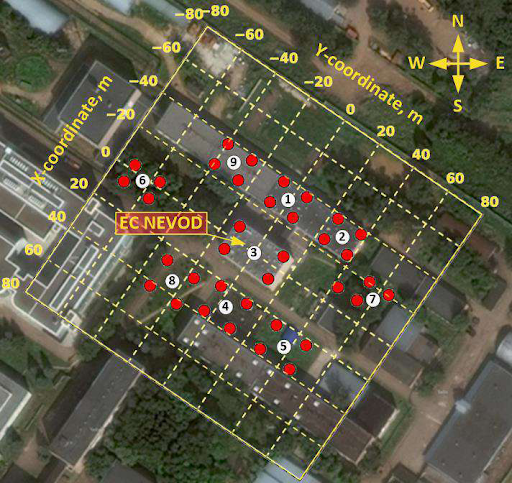
\includegraphics[width=0.95\textwidth, keepaspectratio]{images/невод-шал.png}%
        \label{fig:big_image}%
    }


    % Две маленькие картинки
    \subfloat[]{%
        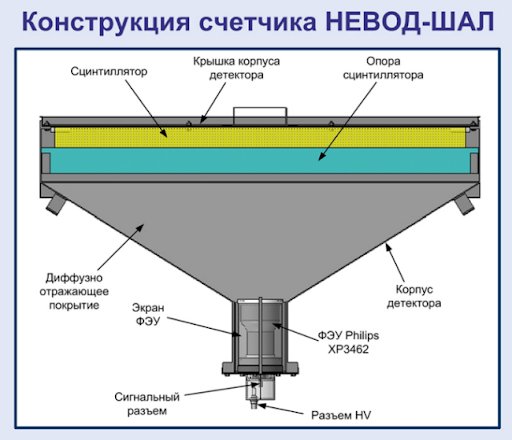
\includegraphics[height=5.2cm, keepaspectratio]{images/счетчик_шал.png}%
        \label{fig:small_image1}%
    }
    \hspace{0.04\textwidth}
    \subfloat[]{%
        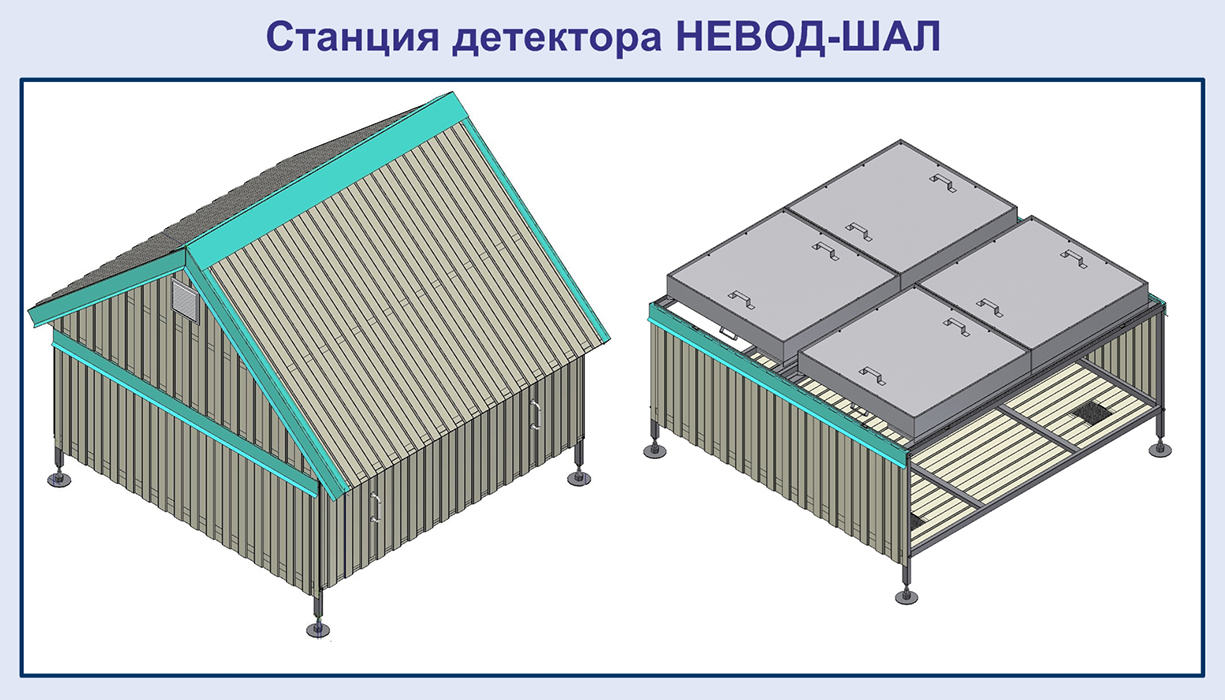
\includegraphics[height=5.2cm, keepaspectratio]{images/ds.jpg}%
        \label{fig:small_image2}%
    }

    \caption{Схема расположения кластеров установки НЕВОД-ШАЛ вокруг ЭК НЕВОД (a), конструкция счетчика (б) и детектирующая станция (a)}
    \label{fig:small_images}
\end{figure}


% Две маленькие картинки с текстом сверху и синей обводкой и тенью





\endinput